\section{Prior Studies}

\begin{frame}{2021 - R. Pelé et al.}

    Title: First Study on Ammonia Spray Characteristics with a Current GDI Engine Injector

    \vspace{9pt}

    \begin{columns}[c, onlytextwidth]

        \begin{column}{0.45\textwidth}

            \begin{figure}[H]
                \centering
                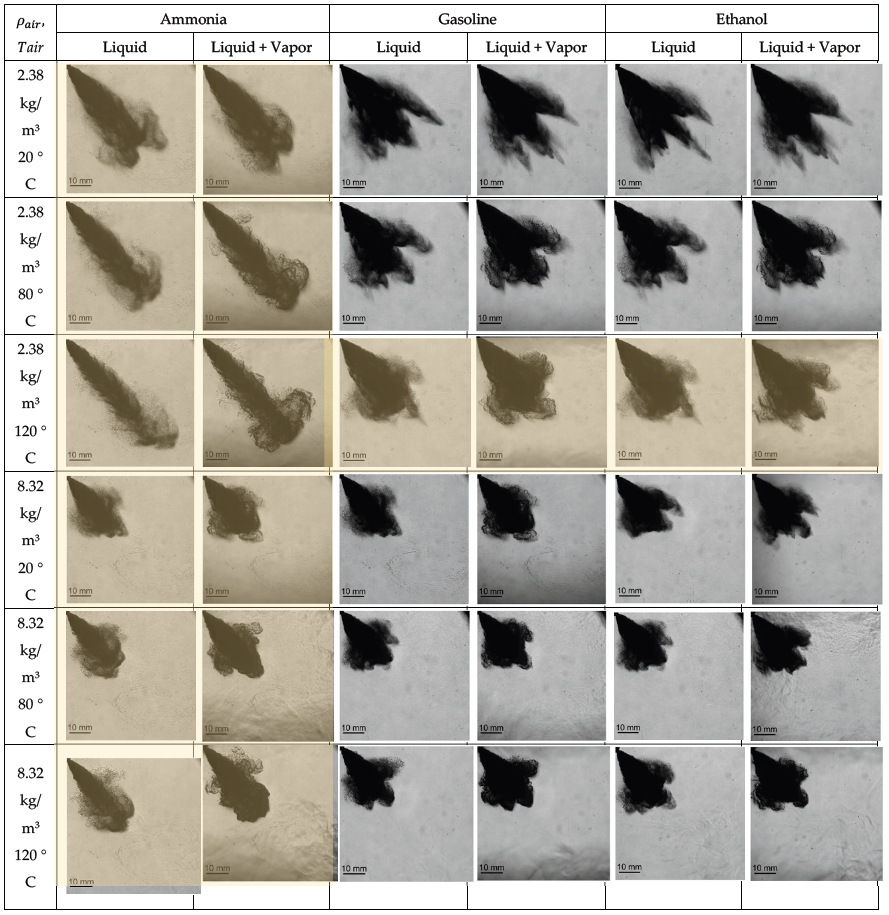
\includegraphics[width=0.8\textwidth]{img/studies-Pele.png}
                \caption{Comparison of spray shape (different fuels \& conditions).}
            \end{figure}

        \end{column}

        \begin{column}{0.5\textwidth}

            Geometrical spray characteristics analysis of Ammonia compared to Gasoline \& Ethanol.

            Conclusions:
            \begin{itemize}
                \item Ammonia spray is longer and thinner.
                \item Spray angle maximum at $P_{sat}$.
                \item Empirical correlation for $spray_L(t)$ proposed.
            \end{itemize}

            In general, the study \textbf{enhanced the possibility for the use of Ammonia} in GDI engines.

        \end{column}

    \end{columns}

\end{frame}



% \begin{frame}{2021 - Y. Fan et al.}
%     Title: Characteristics of Ammonia Spray Injected by Pressure-Swirl Atomizers
% \end{frame}



\begin{frame}{2021 - K.D.K.A. Somarathne et al.}

    Title: Liquid Ammonia Spray Combustion and Emission Characteristics with Gaseous Hydrogen/air Co-firing

    A \textbf{numerical model} for $\mathrm{LNH_3}$\footnotemark[1] combustion was developed and validated (LES\footnotemark[2] based).
    Particular attention to the \textbf{flash-boiling condition} modelling was given.

    \vspace{9pt}

    \begin{figure}[H]
        \centering
        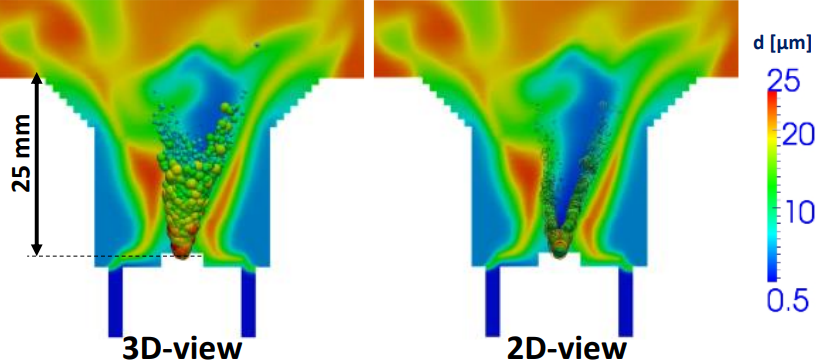
\includegraphics[width=0.6\textwidth]{img/studies-Somarathne.png}
        \caption{3D and 2D views of $\mathrm{LNH_3}$ droplet distributions.}
    \end{figure}

    \footnotetext[1]{LNH3: Liquid Ammonia}
    \footnotetext[2]{LES: Large Eddy Simulation}

\end{frame}



\begin{frame}{2023 - J. Wang, F. Dalla Barba}

    Title: Assessment of the parcel model in evaporating turbulent diluted sprays within a Large-Eddy-Simulation approach

    The \textbf{parcel model} approach was proven to be accurate up to a threshold of the PR\footnotemark[1] number dependent also from the coarsening factor of the grid.

    \vspace{9pt}

    \begin{figure}[H]
        \centering
        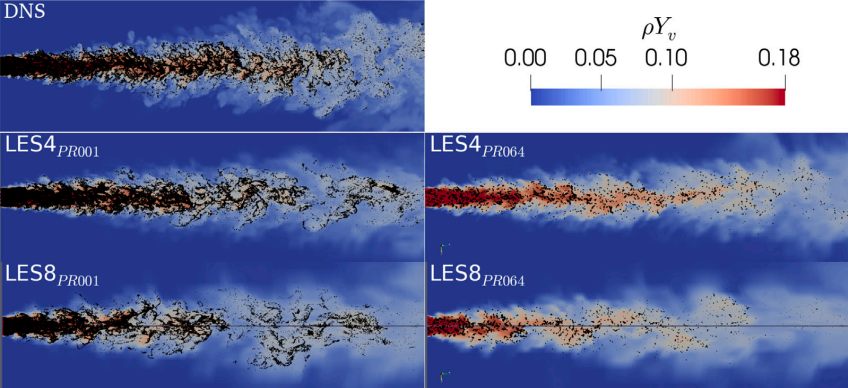
\includegraphics[width=0.8\textwidth]{img/studies-Wang-Dalla-Barba.png}
        \caption{Subset of the simulation runs\footnotemark[2].}
    \end{figure}

    \footnotetext[1]{PR: Parcel Ratio}
    \footnotetext[2]{Here the carrier phase is contoured according to the instantaneous vapor mass fraction field ($\rho Y_v$)}

\end{frame}



\begin{frame}{2023 - J. Wang, F. Dalla Barba}

    The research focused on \textbf{simulating a turbulent diluted acetone jet-spray}.

    \begin{columns}[c, onlytextwidth]

        \begin{column}{0.5\textwidth}

            The numerical model was based on:

            \begin{itemize}
                \item LES framework to simulate turbulence behavior
                \item Hybrid \textbf{Eulerian-Lagrangian technique with two-way coupling}
                \item Parcel model for relaxed droplet tracking
            \end{itemize}

        \end{column}

        \begin{column}{0.5\textwidth}

            \begin{figure}[H]
                \centering
                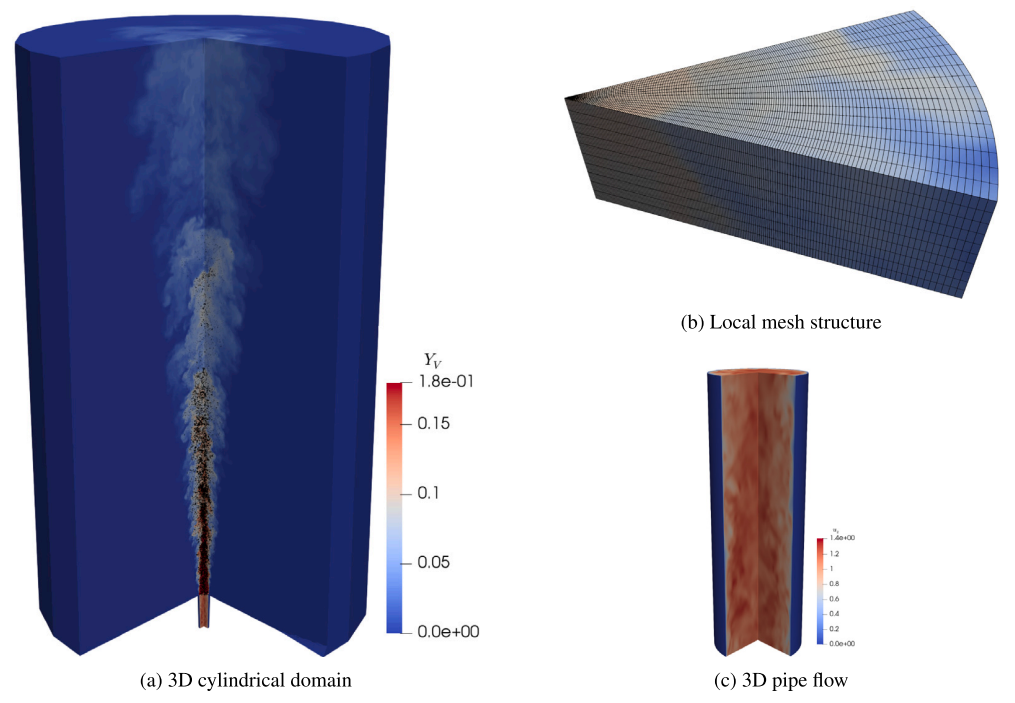
\includegraphics[width=0.9\textwidth]{img/studies-Wang-Dalla-Barba-domain.png}
                \caption{The open-constant pressure-cylindrical domain used for the analysis.}
            \end{figure}

        \end{column}

    \end{columns}

\end{frame}